\documentclass[11pt]{article}
\usepackage{geometry}                % See geometry.pdf to learn the layout options. There are lots.
\geometry{a4paper}                   % ... or a4paper or a5paper or ...
%\geometry{landscape}                % Activate for for rotated page geometry
\usepackage[parfill]{parskip}    % Activate to begin paragraphs with an empty line rather than an indent
\usepackage{setspace}
\usepackage{graphicx}
\usepackage{fullpage}
\usepackage{mhchem}
\usepackage{helvet}
\usepackage{nopageno}
\usepackage{url}

\usepackage[german]{babel}
\usepackage[T1]{fontenc}
\usepackage[utf8]{inputenc}


\DeclareGraphicsRule{.tif}{png}{.png}{`convert #1 `dirname #1`/`basename #1 .tif`.png}

\title{Referat: Akkumulatoren}
\author{Leon Handreke}
\date{}                                           % Activate to display a given date or no date

\begin{document}
\maketitle
\fontfamily{phv}\selectfont
\onehalfspacing

\section{Geschichte}
\begin{itemize}
\item 1789 - Luigi Galvani - Galvanisches Element
\item 1802 - Wilhelm Ritter - Erste ``aufladbare'' Zelle
\item 1850 - Josef Sinsteden - Bleiakkumulator
\item 1866 - Werner von Siemens - Elektrischer Generator
\end{itemize}

\section{Definition}
\begin{quote}
  Ein Akkumulator ist ein Speicher für elektrische Energie, meist auf Basis eines elektrochemischen Systems.
\end{quote}
\small{Wikipedia}


\section{Bleiakku}
\begin{itemize}
\item Elektrolyt: Schwefelsäure (\ce{H2SO4})
\item Spannung: 2V
\item Pluspol: \ce{PbO2}
\item Minuspol: \ce{Pb}
\end{itemize}

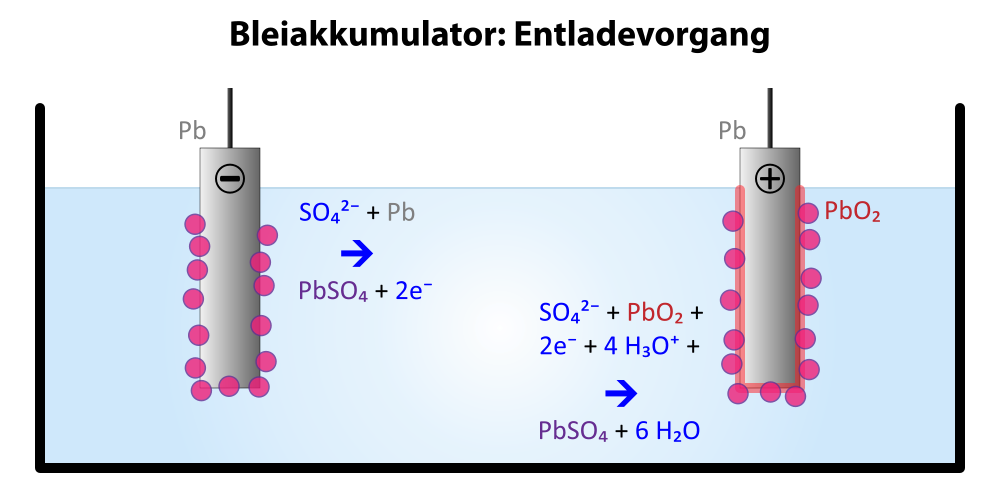
\includegraphics[width=\textwidth]{bleiakku-entladung.png}

\section{Spannung}
  $\Delta EMK = E ^{0} _{A} - E ^{0} _{D}$

Für das Beispiel des Bleiakkus:

  $\Delta EMK = E ^{0} _{\ce{Pb4+}} - E ^{0} _{\ce{Pb}}$ \\
  $\Delta EMK = 1.8V - (-0.1262V) = 2V$

\section{Andere Akkumulatortypen}
\begin{itemize}
\item Nickel-Cadmium
  \begin{itemize}
  \item Giftig, Verkaufsverbot in der EU
  \end{itemize}
\item Nickel-Metallhydrid
\item Lithium-Ionen
\item Lithium-Polymer
  \begin{itemize}
  \item Sehr leicht und teuer
  \end{itemize}
\end{itemize}

\section{Quellen}
\begin{itemize}
\item \url{http://www.u-helmich.de/che/09/04-ionen/ionen14.html}
\item \url{http://de.wikipedia.org/wiki/Akkumulator}
\item \url{http://de.wikipedia.org/wiki/Bleiakkumulator}
\item \url{http://commons.wikimedia.org/} (Illustrationen)
\end{itemize}


\end{document}
